% FILE: figures/gradient_osmosis_tension.tex
% Gradients and osmotic tension

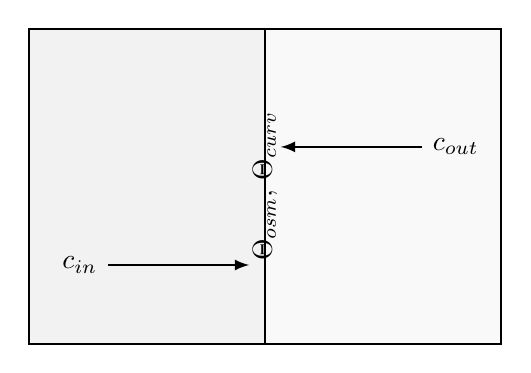
\begin{tikzpicture}[>=latex,thick,scale=1]
  % Membrane
  \draw[thick] (0,0) -- (0,4);

  % Left compartment (inside)
  \node at (-1.5,3.5) {inside};
  \draw[fill=gray!10] (-3,0) rectangle (0,4);

  % Right compartment (outside)
  \node at (1.5,3.5) {outside};
  \draw[fill=gray!5] (0,0) rectangle (3,4);

  % Concentration gradients (arrows)
  \draw[->] (-2.0,1.0) -- (-0.2,1.0);
  \node[anchor=east] at (-2.0,1.0) {$c_{\text{in}}$};

  \draw[->] (2.0,2.5) -- (0.2,2.5);
  \node[anchor=west] at (2.0,2.5) {$c_{\text{out}}$};

  % Tension label
  \node[rotate=90] at (0,2.0) {$\Theta_{\text{osm}}$, $\Theta_{\text{curv}}$};
\end{tikzpicture}
